\chapter{Progettazione e codifica}
\label{cap:progettazione-codifica}

\intro{Questo capitolo tratta della fase di progettazione e della fase di codifica dell'app, riportando tutto quello che è stato fatto e le difficoltà incontrare.}\\ %-----------------------------------------------------------------------------------------------------------------------------------------------------------------------------------------------------------------------------------------------------------

\section{Progettazione}
\label{sec:progettazione}

\subsection{Struttura dell'app}

Dopo una prima parte di stage, dove ho studiato le tecnologie riportare al \hyperref[sec:tecnologie]{secondo capitolo}, ho pensato come sviluppare l'applicazione richiesta.\newline
Di prassi in RiskAPP si utilizza Figma per poter avere una idea più chiara del lavoro che si desidera fare, quindi per prima cosa ho progettato la grafica e la struttura dell'app con l'aiuto di questo software di progettazione.\newline
Avendo una idea visiva, questo rendeva più facile spiegare al mio tutor come pensavo di impostare l'applicazione, andando poi a modificare e sistemare in base alle esigenze dell'azienda.\newline
\newline
Nella Figura \ref{fig:schermatefigma} ci sono tre schermate progettate in Figma, ovvero le schermate \textbf{Utente}, \textbf{Impostazioni} e infine \textbf{Home}.\newline
Dai \emph{mockup} capiamo che la struttura delle pagine è la seguente:
\begin{itemize}
    \item una barra superiore, dove è possibile eseguire una o due azioni;
    \item una schermata con le informazioni interessate;
    \item una barra inferiore che permette di navigare tra le schermate, fatta eccezzione per la schermata \textbf{Impostazioni} che non ha questa barra.
\end{itemize}
Tramite la barra inferiore è possibile navigare tra le schermate:
\begin{itemize}
    \item \textbf{Home} dove sarà visibile la \emph{\gls{cassacomuneg}}, la \emph{\gls{quotastornatag}} dell'utente e infine il piatto del giorno (successivamente cambiato in \emph{Proposte del giorno} per permettere la scelta di più piatti dal menu);
    \item \textbf{Spese} che permette di visualizzare tutte le transazioni di tutti gli utenti e aggiungere delle nuove transazioni o eliminarle;
    \item \textbf{Menu} dove è possibile consultare i piatti, aggiungerli oppure proporli come possibili piatti del giorno;
    \item \textbf{Utente} la visualizzazione cambia tra utente semplice e utente amministratore ed è stata modificata durante la fase di codifica, ma principalmente serve per visualizzare e modificare le proprie presenze o, nel caso dell'amministratore, visualizzare e modificare le presenze degli stagisti o della \emph{\gls{quotapastog}}.
\end{itemize}
\begin{figure}[!h]
    \centering 
    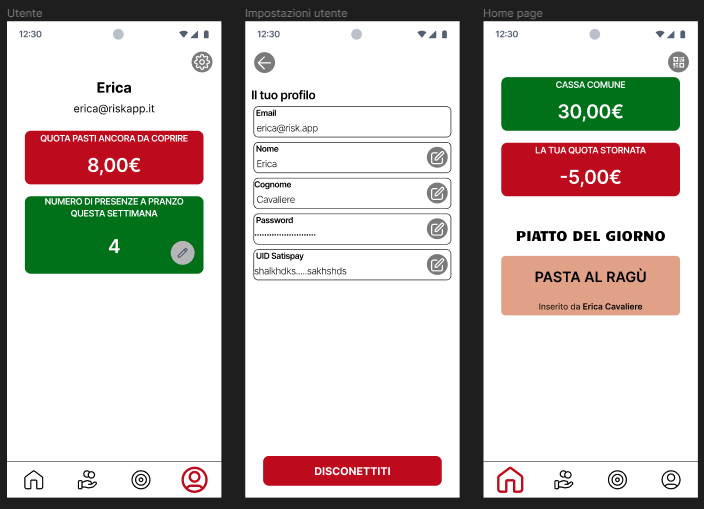
\includegraphics[width=0.9\columnwidth]{figma/esempi} 
    \caption{Alcune schermate progettate in Figma}
    \label{fig:schermatefigma}
\end{figure}
La schermata \textbf{Impostazioni} è raggiungibile attraverso la schermata \textbf{Utente}, andando a toccare l'icona ad ingranaggio posta nella barra superiore.\newline
Da \textbf{Impostazioni} è possibile modificare i dati dell'utente oppure permettere all'utente di disconnettersi dalla sessione corrente.\newline
\newline
Sono state create diversamente anche le finestre \textbf{Accedi} (Figura \ref{fig:accedifigma}) e \textbf{Registrati} (Figura \ref{fig:registratifigma}).\newline
In queste due schermate non sono presenti barre superiori o inferiori, ma solo una serie di campi da compilare e il pulsante verde Accedi o Registrati.\newline
\textbf{Accedi} è la prima schermata che vede l'utente quando entra nell'app per la prima volta; per passare alla schermata \textbf{Registrati} bisogna toccare il link presente sotto al pulsante Accedi, dove è scritto il messaggio "\emph{Sei nuovo? REGISTRATI}".\newline
Per ritornare alla schermata \textbf{Accedi}, il procedimento è analogo, ovvero si tocca il link presente sotto il pulsante Registrati, dove è riportato il messaggio "\emph{Hai già un account? ACCEDI}".\newline
Invece, per andare in \textbf{Home}, bisognerà compilare correttamente i campi e poi toccare il pulsante verde presente.\newline
\newline
In \textbf{Accedi} è presente il messaggio "\emph{Hai dimenticato la password?}", questo doveva contenere un link che permetteva all'utente di recuperare la propria password, ma poi è stato tolto, in accordo con il tutor, perchè non aveva alcuna utilità.\newline
%qui poi si dovrà riportare le schermate a 0.7 in base all'introduzione ---------------------------------------------------------------------------------------------------------------------------------------------------------------------
\begin{figure}[!h] 
    \centering 
    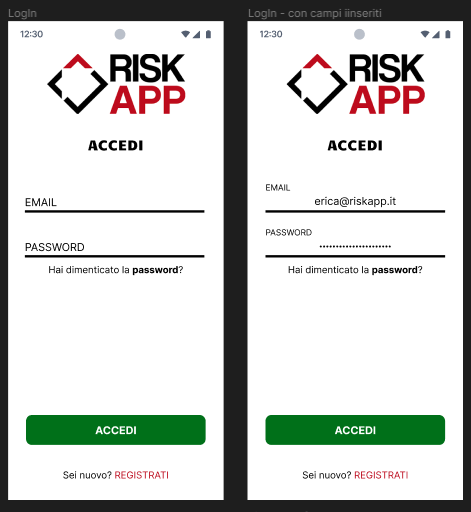
\includegraphics[width=0.6\columnwidth]{figma/accedi} 
    \caption{Schermata Accedi progettata in Figma}
    \label{fig:accedifigma}
\end{figure}
\begin{figure}[!h] 
    \centering 
    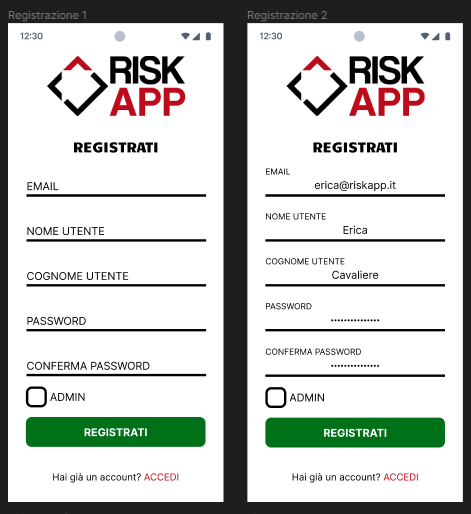
\includegraphics[width=0.6\columnwidth]{figma/registrati} 
    \caption{Schermata Registrati progettata in Figma}
    \label{fig:registratifigma}
\end{figure}
%Come è già stato detto, sono state fatte diverse modifiche in fase di progettazione, alcune modifiche sono state fatte perchè non rispettavano le idee del proponente, altre perchè non avevano utilità, come il recupero password appena accennato, altre modifiche sono state fatte anche a livello grafico, perchè non permetteva all'utente di capire che cosa poteva fare.\newline
%Per questo sono state fatte delle modifiche anche ai componenti utilizzati (nella figura \ref{fig:conteinerfigma} ci sono i \emph{component} creati per il \emph{mockup}), pure le icone dei pulsanti, che servivano solo a livello dimostrativo.
%\begin{figure}[!h] 
%    \centering 
%    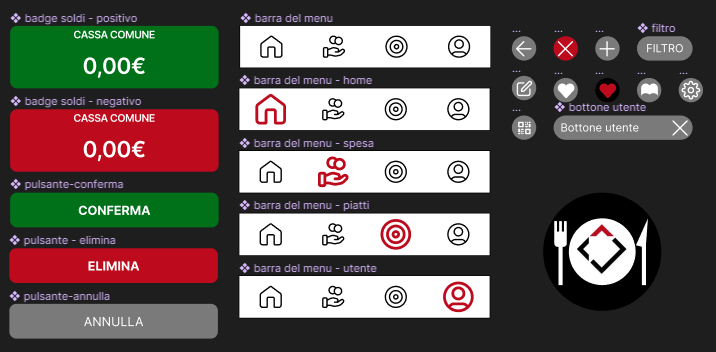
\includegraphics[width=0.9\columnwidth]{figma/container} 
%    \caption{Alcuni pulsati e icone progettate in Figma}
%    \label{fig:conteinerfigma}
%\end{figure}

\newpage

\subsection{Database}

\begin{figure}[!h] 
    \centering 
    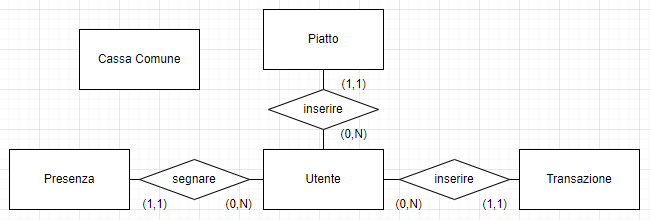
\includegraphics[width=0.9\columnwidth]{database} 
    \caption{Il database progettato per l'applicazione}
    \label{fig:database}
\end{figure}

\newpage

\section{Design Pattern utilizzati}
%forse parlare dell'MVVM o BLoC patttern

\section{Codifica} %riportare qui il database?
%In questa sezione riporto la struttura della cartella lib, parlerò delle componenti e, del file firebase_option e delle classi
%riportare anche le immagine dell'app creata